\documentclass{article}

% Language setting
% Replace `english' with e.g. `spanish' to change the document language
\usepackage[english]{babel}
\usepackage{caption}
% Set page size and margins
% Replace `letterpaper' with`a4paper' for UK/EU standard size
\usepackage[letterpaper,top=2cm,bottom=2cm,left=3cm,right=3cm,marginparwidth=1.75cm]{geometry}

% Useful packages
\usepackage{amsmath}
\usepackage{graphicx}
\usepackage{authblk} % this is for multiple autho  rs 
\usepackage[colorlinks=true, allcolors=blue]{hyperref}
\usepackage{cleveref}
\usepackage{booktabs}
\usepackage{multirow}

% Configure for "Fig.":
\crefname{figure}{Fig.}{Figs.}
\Crefname{figure}{Fig.}{Figs.}


% reference configuration
\usepackage[authoryear,round]{natbib}
\bibliographystyle{apalike} % for an APA-like style
\usepackage{amsmath}

% reference configuration
\usepackage[authoryear,round]{natbib}
\bibliographystyle{apalike} % for an APA-like style

%%%%%%%%%%%%%%%%%%%%%%%%%%%%%%%%%%%%
%%% --- Tittle of the paper --- %%%
%%%%%%%%%%%%%%%%%%%%%%%%%%%%%%%%%%
\title{\textbf{Supplementary materials: Development of outdoor air pollution models for estimating exposure in the Barcelona Life Study Cohort (BiSC)}}

%%%%%%%%%%%%%%%%%%%%%%%%%%%%%%%%%%%%%%%%%
%%% --- Authors and affiliations --- %%%
%%%%%%%%%%%%%%%%%%%%%%%%%%%%%%%%%%%%%%%

%%% --- Authors --- %%%
\author{Alan Domínguez, Payam Dadvand, Marta Cirach, Bruno Raimbault, Toni Galmes, Karl Samuelsson, Mark Nieuwenhuijsen, Jordi Sunyer, Xavier Basagaña, Ioar Rivas}
%%%%%%%%%%%%%%%%%%%%%%%%%%%%%%%%%%%%%%%%%%%%%%%%%%%%%%%%%%%%%%%%%%%%%%%%%

\begin{document}
\maketitle

%%%%%%%%%%%%%%%%%%%%%%%%%%%%%%%%%%%%%%%%%%%%%%
%%% --- Land Use Regression modelling --- %%% 
%%%%%%%%%%%%%%%%%%%%%%%%%%%%%%%%%%%%%%%%%%%%
\section{Land Use Regression modelling details}

\subsection{Predictor variables and sources of information}

\subsection{Performance metrics}
The following metrics were used to evaluate the LUR model for all the air pollution assessed. 



% --- R2 --- %
\begin{equation}
R^2 = \left( \frac{\sum (\hat{y}_i - \bar{y})^2}{\sum (y_i - \bar{y})^2} \right)
\end{equation}

% --- root mean squared error (RMSE) --- % 
\begin{equation}
\text{RMSE} = \sqrt{\frac{1}{n} \sum_{i=1}^{n} (y_i - \hat{y}_i)^2}
\end{equation}

% --- mean bias (MB) --- % 
\begin{equation}
\text{Mean Bias} = \frac{1}{n} \sum_{i=1}^{n} (y_i - \hat{y}_i)
\end{equation}

% --- correlation coefficient (r) --- %
\begin{equation}
r = \frac{\sum (x_i - \bar{x})(y_i - \bar{y})}{\sqrt{\sum (x_i - \bar{x})^2 \sum (y_i - \bar{y})^2}}
\end{equation}
\vspace{0.5 cm}


\subsection{Model performance}



\newpage
%%%%%%%%%%%%%%%%%%%%%%%%%%%%%%%%%%%%%
%%% --- Dispersion modelling --- %%% 
%%%%%%%%%%%%%%%%%%%%%%%%%%%%%%%%%%%%


\section{Dispersion modelling details}

\subsection{Predictor variables and sources of information}

\subsection{Performance metrics}

\subsection{Model performance}


\newpage
%%%%%%%%%%%%%%%%%%%%%%%%%%%%%%%%%
%%% --- Hybrid modelling --- %%%%%%%%%%%%%%%%%%%%%%%%%%%%%%%%%%%%%%%%%%%%%%
%%%%%%%%%%%%%%%%%%%%%%%%%%%%%%%

\section{Hybrid modelling details}

\subsection{Predictor variables and sources of information}


\subsection{Performance metrics}


\subsection{Model performance}

%%% --- Table with performance metrics for Hybrid models --- %%%
\begin{table}[ht]
\centering
\caption{Performance metric for hybrid models.}
\begin{tabular}{llllll}
\toprule
\textbf{Dataset campaign} & \textbf{Pollutant} & \textbf{N} & \textbf{R\textsuperscript{2} (10-CV)} & \textbf{RMSE (10-CV)} \\
\midrule
BiSC-home & NO\textsubscript{2} & 1232 & 0.64 & 7.48 \\
\multirow{5}{*}{BiSCAPE} & PM\textsubscript{2.5} & 161 & 0.66 & 3.45 \\
& BC & 74 & 0.86 &  0.23 \\
& Fe & ... & 0.54 & ... \\
& Cu & ... & 0.70 & ... \\
& Zn & ... & 0.42 & ... \\
\bottomrule
\end{tabular}
\label{tablesX}
\end{table}


\subsection{Variable importance}

%%% --- Figure. Comparison between measurements and predictions values in the test dataset --- %%%
% Put the figure text closer to the Figure 3
\captionsetup[figure]{skip=6pt}
% We add the figure with the study domain 
\begin{figure}[!htb]
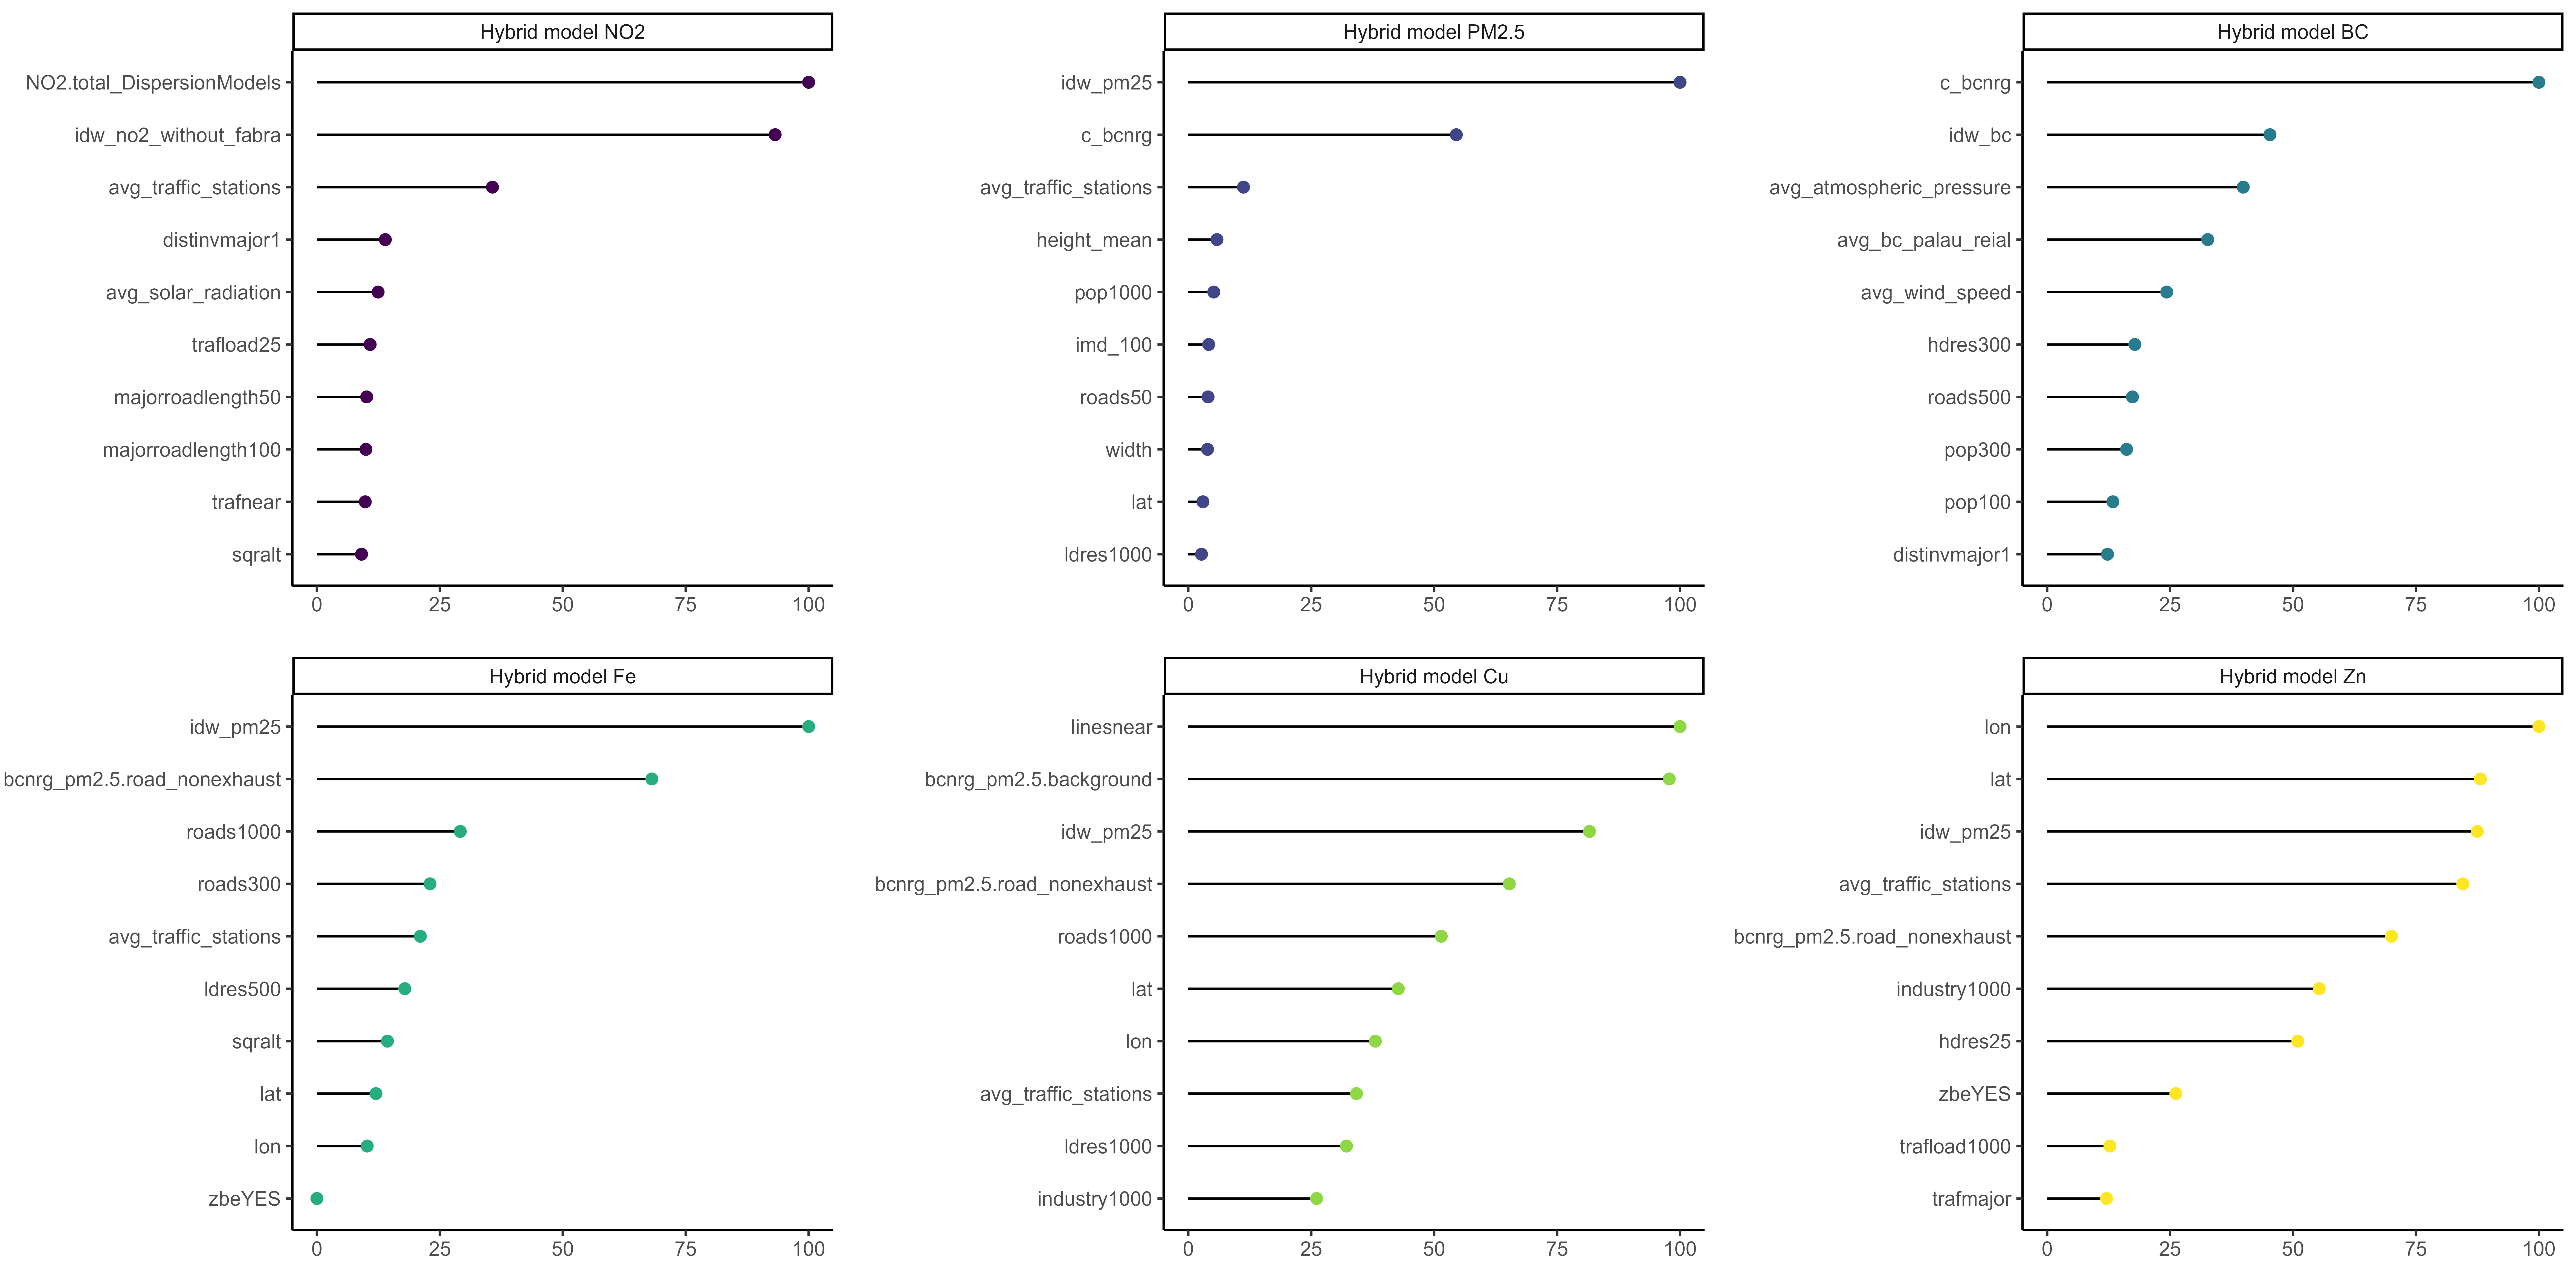
\includegraphics[width=1.0\textwidth]{figures/fig_HM_allmodels_importance.png}
\caption{Comparison between measurements and prediction values for the hybrid models for \textit{NO$_2$}, \textit{PM$_{2.5}$}, \textit{BC}, \textit{Fe}, \textit{Cu} and \textit{Zn}.}
\label{fig2}
\end{figure}

\newpage

\subsection{Comparison between observed measurements and predictions}

%%% --- Figure. Comparison between measurements and predictions values in the test dataset --- %%%
% Put the figure text closer to the Figure 3
\captionsetup[figure]{skip=6pt}
% We add the figure with the study domain 
\begin{figure}[!htb]
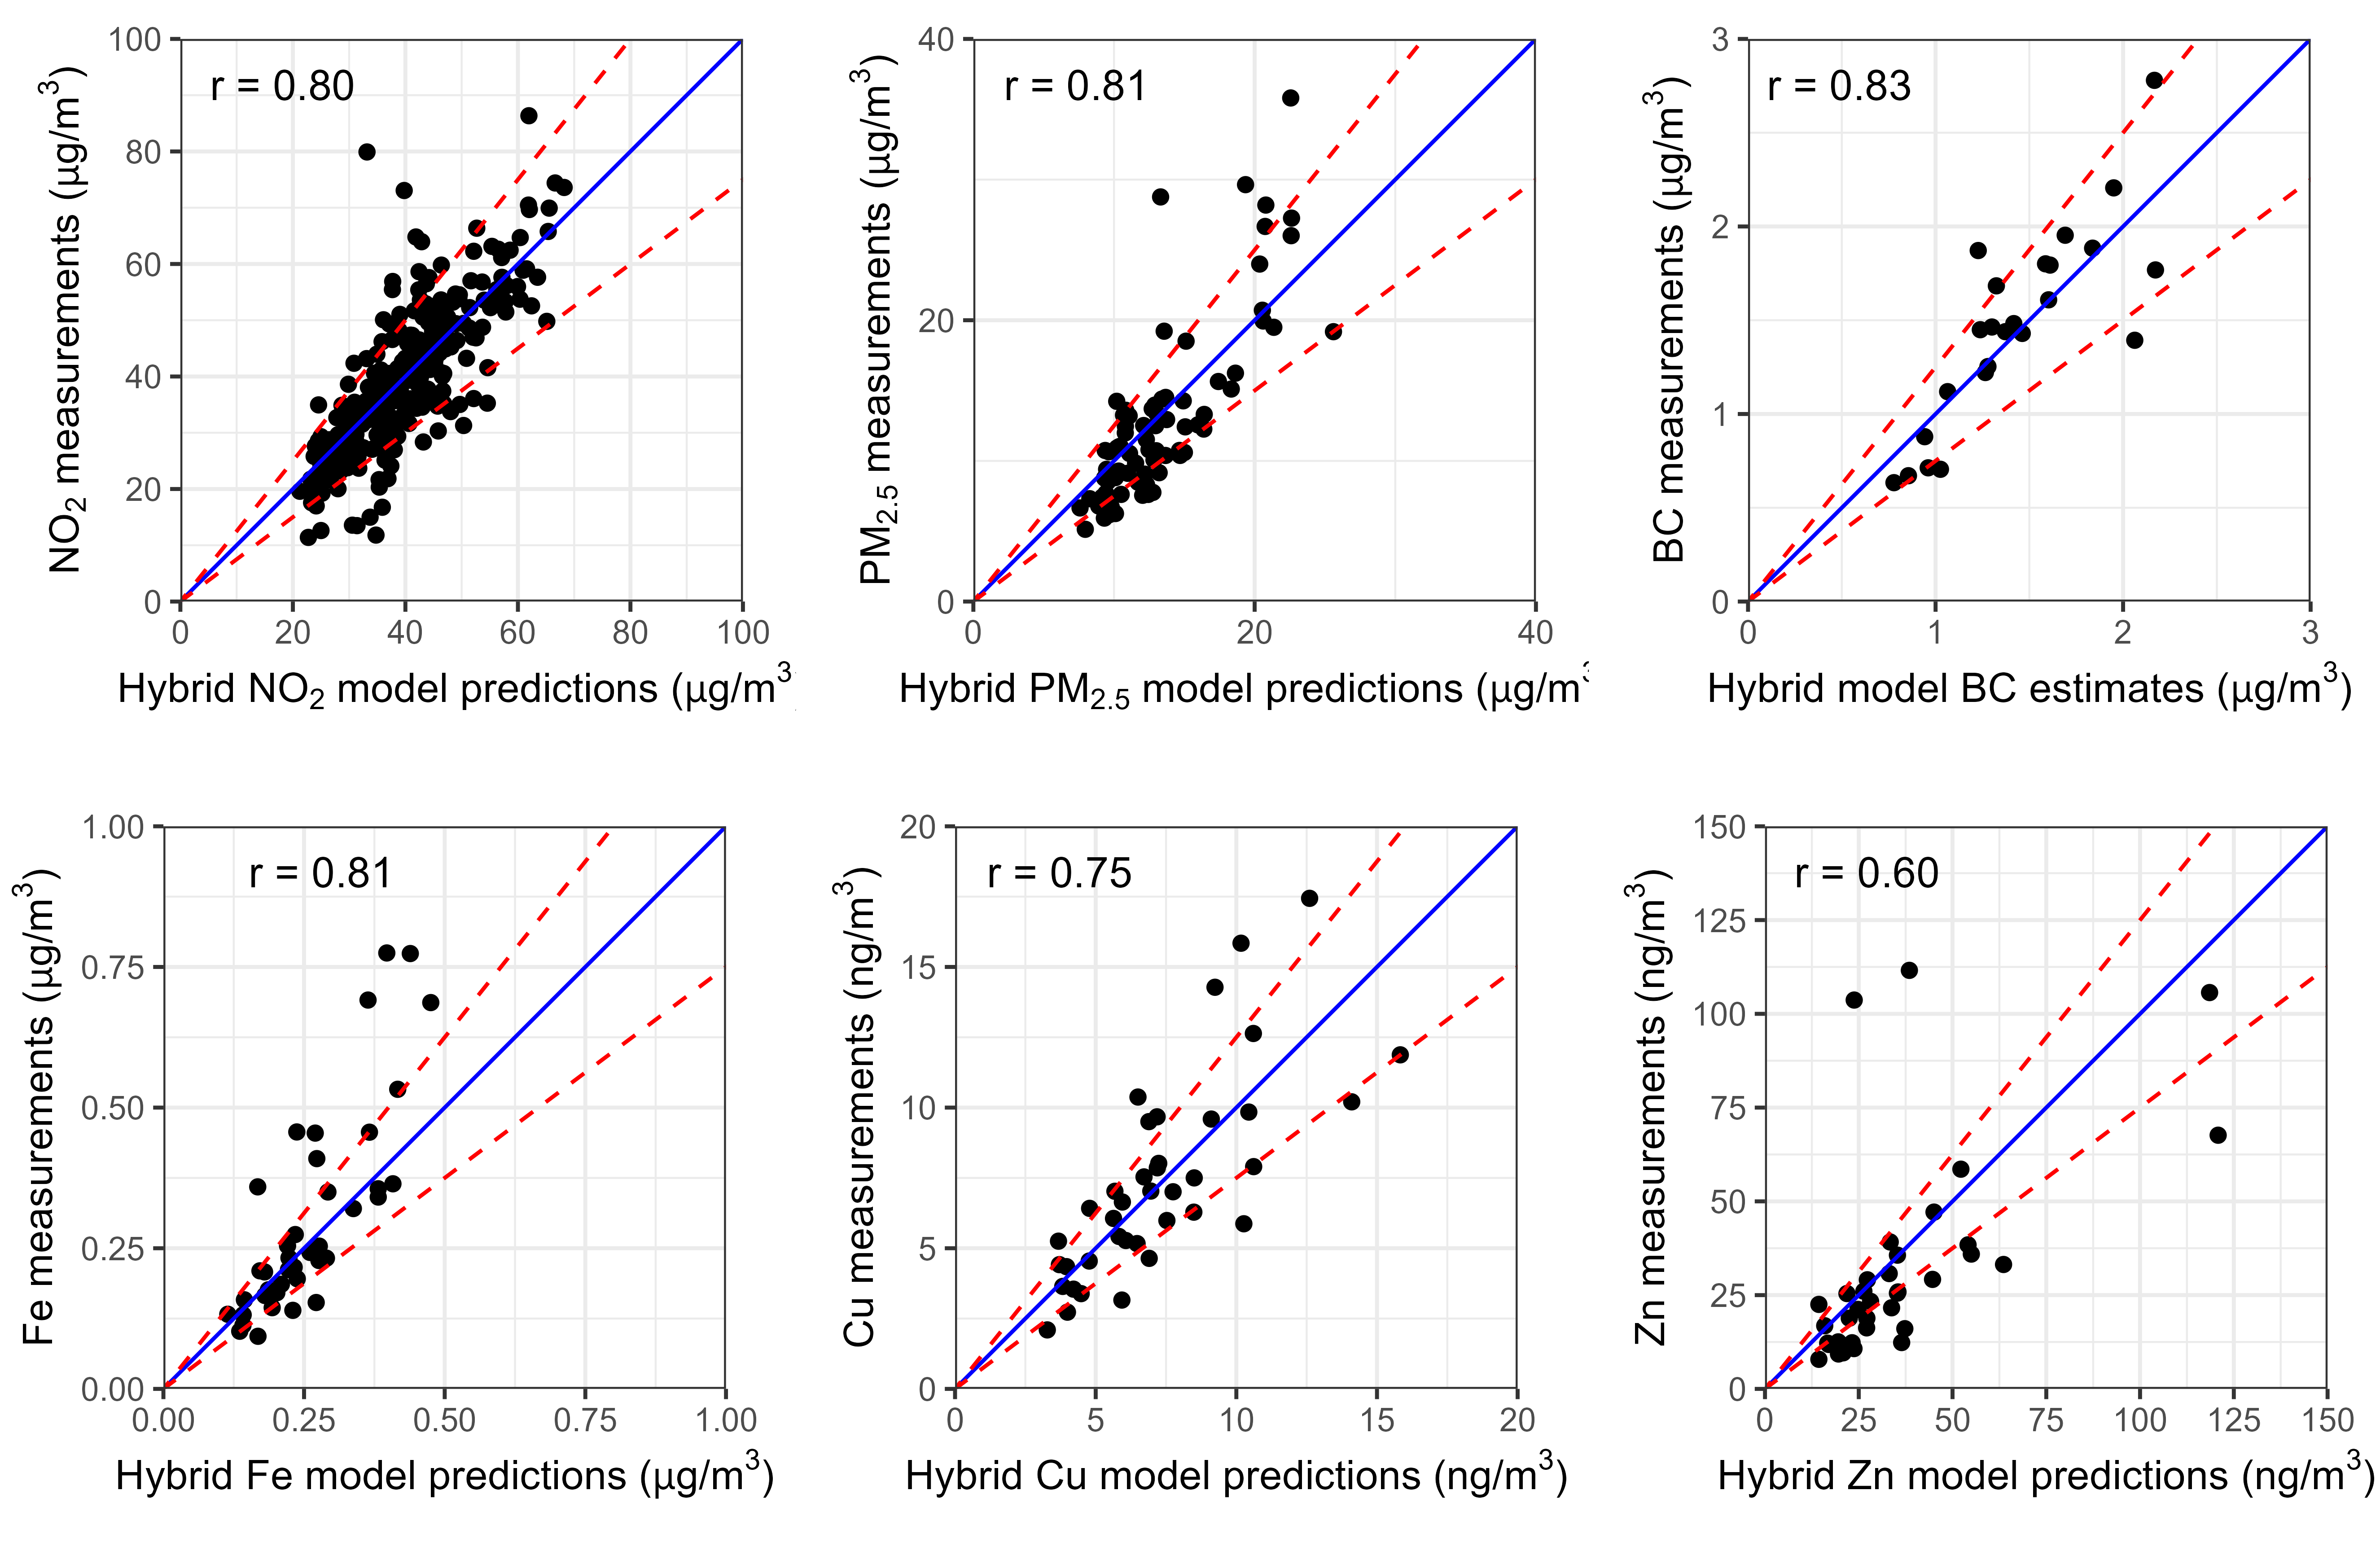
\includegraphics[width=1.0\textwidth]{figures/fig_HM_test_all_models.png}
\caption{Comparison between measurements and prediction values for the hybrid models for \textit{NO$_2$}, \textit{PM$_{2.5}$}, \textit{BC}, \textit{Fe}, \textit{Cu} and \textit{Zn}.}
\label{fig2}
\end{figure}







%%%%%%%%%%%%%%%%%%%%%%%%%%%
%%% --- References --- %%%
%%%%%%%%%%%%%%%%%%%%%%%%%%%

\bibliography{references}


\end{document}